%%%%%%%%%%%%%%%%%%%%%%%%%%%%%%%%%%%%%%%%%%%%%%%%%%%%%%%%%%%%%%%%%%%%%%%%%%%%%%%%%%%%%%%
%%%%%%%%%%%%%%%%%%%%%%%%%%%%%%%%%%%%%%%%%%%%%%%%%%%%%%%%%%%%%%%%%%%%%%%%%%%%%%%%%%%%%%%
% 
% This top part of the document is called the 'preamble'.  Modify it with caution!
%
% The real document starts below where it says 'The main document starts here'.

\documentclass[12pt]{article}

\usepackage{amssymb,amsmath,amsthm}
\usepackage[top=1in, bottom=1in, left=1.25in, right=1.25in]{geometry}
\usepackage{fancyhdr}
\usepackage{graphicx}
\usepackage{enumerate}
\usepackage{verbatim}
\usepackage{listings}

% Comment the following line to use TeX's default font of Computer Modern.
\usepackage{times,txfonts}

\newtheoremstyle{homework}% name of the style to be used
  {18pt}% measure of space to leave above the theorem. E.g.: 3pt
  {12pt}% measure of space to leave below the theorem. E.g.: 3pt
  {}% name of font to use in the body of the theorem
  {}% measure of space to indent
  {\bfseries}% name of head font
  {:}% punctuation between head and body
  {2ex}% space after theorem head; " " = normal interword space
  {}% Manually specify head
\theoremstyle{homework} 

% Set up an Exercise environment and a Solution label.
\newtheorem*{exercisecore}{\@currentlabel}
\newenvironment{exercise}[1]
{\def\@currentlabel{#1}\exercisecore}
{\endexercisecore}

\newcommand{\localhead}[1]{\par\smallskip\noindent\textbf{#1}\nobreak\\}%
\newcommand\solution{\localhead{Solution:}}



% \newcommand{includematlab}[1]{\verbatiminput{#1}}

%%%%%%%%%%%%%%%%%%%%%%%%%%%%%%%%%%%%%%%%%%%%%%%%%%%%%%%%%%%%%%%%%%%%%%%%
%
% Stuff for getting the name/document date/title across the header
\makeatletter
\RequirePackage{fancyhdr}
\pagestyle{fancy}
\fancyfoot[C]{\ifnum \value{page} > 1\relax\thepage\fi}
\fancyhead[L]{\ifx\@doclabel\@empty\else\@doclabel\fi}
\fancyhead[C]{\ifx\@docdate\@empty\else\@docdate\fi}
\fancyhead[R]{\ifx\@docauthor\@empty\else\@docauthor\fi}
\headheight 15pt

\def\doclabel#1{\gdef\@doclabel{#1}}
\doclabel{Use {\tt\textbackslash doclabel\{MY LABEL\}}.}
\def\docdate#1{\gdef\@docdate{#1}}
\docdate{Use {\tt\textbackslash docdate\{MY DATE\}}.}
\def\docauthor#1{\gdef\@docauthor{#1}}
\docauthor{Use {\tt\textbackslash docauthor\{MY NAME\}}.}
\makeatother

%% General formatting parameters
\parindent 0pt
\parskip 12pt plus 1pt

\def\vx{\mathbf x}
\def\vb{\mathbf b}

% Shortcuts for blackboard bold number sets (reals, integers, etc.)
\newcommand{\Reals}{\ensuremath{\mathbb R}}
\newcommand{\Nats}{\ensuremath{\mathbb N}}
\newcommand{\Ints}{\ensuremath{\mathbb Z}}
\newcommand{\Rats}{\ensuremath{\mathbb Q}}
\newcommand{\Cplx}{\ensuremath{\mathbb C}}
%% Some equivalents that some people may prefer.
\let\RR\Reals
\let\NN\Nats
\let\II\Ints
\let\CC\Cplx

%%%%%%%%%%%%%%%%%%%%%%%%%%%%%%%%%%%%%%%%%%%%%%%%%%%%%%%%%%%%%%%%%%%%%%%%%%%%%%%%%%%%%%%
%%%%%%%%%%%%%%%%%%%%%%%%%%%%%%%%%%%%%%%%%%%%%%%%%%%%%%%%%%%%%%%%%%%%%%%%%%%%%%%%%%%%%%%
% 
% The main document start here.

% The following commands set up the material that appears in the header.

%%%%%%%%%%%%%%%%%%%%%%%%%%%%%%%%%%%%%%%%%%%%%%%%%%%%%%%%%%%%%%%%%%%%%%%%%%
\doclabel{Math 426: Homework 9}
\docauthor{Stefano Fochesatto}
\docdate{October 28, 2020}

\begin{document}

\begin{exercise}{Exercise 7.9} Compute the $1-norm$ and $\infty-norm$ of the following matrix,
  \begin{equation*}
    A  = \begin{pmatrix}
      5 && 6\\
      7 && 8
    \end{pmatrix}
  \end{equation*}
  Also compute the condition number $k(A) = ||A|| \cdot ||A^{-1}||$ in the $1-norm$ and $\infty-norm$.
  \solution From class we proved that the $1-norm$ of the matrix $A$ is simply the maximum $1-norm$ of the column vectors, so we get 
  that $||A||_1 = 14$. We also showed in class that the $\infty-norm$ of a matrix $A$ is the maximum $1-norm$ of the row vectors, so we get
  $||A||_\infty = 15$. Computing the inverse of $A$,
  \begin{equation*}
    A^{-1} = \dfrac{1}{40 - 42}
    \begin{pmatrix}
      8 && -6\\
      -7 && 5
    \end{pmatrix}
     = \begin{pmatrix}
      -4 && 3\\
      3.5 && -2.5
    \end{pmatrix}.
  \end{equation*}
Computing the norms for $A^{-1}$ we get that $||A^{-1}||_{1} = 7.5$ and $||A^{-1}||_{\infty} = 7$. Therefore we get the following condition numbers
\begin{equation*}
  k(A)_1 = 7.5*14 = 105,
\end{equation*}
\begin{equation*}
  k(A)_{\infty} = 7*15 = 105.
\end{equation*}
\end{exercise}
\vspace{.5in}








\begin{exercise}{Exercise 7.10} Show that for all $n$-vectors $v$,\\

  \begin{enumerate}
    \item $||v||_{\infty} \le ||v||_{2} \le \sqrt{n}||v||_{\infty}$
    \solution Note that for every non empty $v$ there exists some $v_j$ such that,
    \begin{equation*}
      |v_j| \geq |v_n|,
    \end{equation*}
    for all $v_n$; there must exists a maximum vector element. Now the following expression follows expression,
    \begin{equation*}
      v_j^2 \le \sum_{i = 1}^n v_i^2 \le nv_j^2 
    \end{equation*}
    Where $v_j^2$ must be the smallest form the sum of the squares can take on, and $nv_j^2$ begin the largest. Taking the positive square root of the 
    expression,  
    \begin{equation*}
      |v_j| \le (\sum_{i = 1}^n v_i^2)^{\frac{1}{2}} \le n^{\frac{1}{2}}|v_j|, 
    \end{equation*}
    Which is equivalent to the following,
    \begin{equation*}
      ||v||_{\infty} \le ||v||_{2} \le \sqrt{n}||v||_{\infty}.
    \end{equation*}
     \vspace{.25in}

     \item $||v||_{2} \le \sqrt{n}||v||_{1}$\\
     Start with an induction/triangle inequality argument to show that for any number of $n$, real numbers $x_i$
     \begin{equation*}
       x_1^2 + x_2^2 + \cdots + x_n^2 \le (|x_1| + |x_2| + \cdots + |x_n|)^2.
     \end{equation*}\
     Then it follows by the definition of the $1$ and $2$ norms. 
     \vspace{.25in}
    
     \item $||v||_{1} \le n||v||_{\infty}$\\
     Substituting the definitions we get that,
     \begin{align*}
      ||v||_{1} &\le n||v||_{\infty},\\
      (|x_1| + |x_2| + \cdots + |x_n|) &\le n \max\{|x_n|\}.
     \end{align*}
     Clearly this is true.
  \end{enumerate}
  
\end{exercise}
\vspace{.5in}





\begin{exercise}{Exercise 7.14} Find the polynomial of degree 10 which best fits the function $b(t) = cos(4t)$ at 50
  equally spaced points $t$ between 0 and 1. Set up the matrix $A$ and right-hand side vector $b$, and determine 
  the polynomial coefficients in two different ways,\\

  \begin{enumerate}
    \item By using the Matlab command $x = A\/b$.\\
    
    \textbf{Console:}
    \begin{center}
    \lstinputlisting{polyfit.txt}
    \end{center}
  From here we have vector $c$ which lists the coefficients of our polynomial in ascending order of degree, i.e we would use 
  $polyval(c')$.
  \vspace{.25in}

    \item By solving the normal equations $A^{T}Ax = A^Tb$.\\
  
    \textbf{Console:}
    \begin{center}
    \lstinputlisting{polyfitnormal.txt}
    \end{center}
    We have demonstrated in class that solving for the coefficient using the normal equations leads to more error since the condition number of 
    $A^TA$ is the square of $R$ where $A = QR$. Recall that solving the system through $QR$ decomposition with the backslash operator in Matlab means matlab is solving the following,
    \begin{equation*}
      Rc = Q^Tb.
    \end{equation*}
    Similarly when we solve the normal equations with the backslash operator in Matlab we solve the follow system,
    \begin{equation*}
      R_nc = Q_n^Tb.
    \end{equation*}
Where $A^TA = Q_nR_n$ then comparing the condition numbers of $R_n$ and $R$ we see that solving the normal equations leads to a more ill conditioned system and thus less precision.
  
\textbf{Console:}
\begin{center}
\lstinputlisting{condition.txt}
\end{center}
\end{enumerate}
\end{exercise}






\begin{exercise}{Supplemental 1}
Let
\[
A=\begin{pmatrix}  
1 & -1 & 0 & \alpha-\beta & \beta\\
0 & 1 & -1 & 0 & 0\\
0 & 0 & 1 & -1 & 0\\
0 & 0 & 0 & 1 & -1\\
0 & 0 & 0 & 0 & 1 
\end{pmatrix}; \qquad \vb = \begin{pmatrix} \alpha \\0\\0\\0\\1\end{pmatrix}
\]
\begin{enumerate}[a)]
\item Show that that for any choice of numbers $\alpha$ and $\beta$, 
the solution of $A\vx=\vb = (1,1,1,1,1)^T$.\\

\solution Performing a simple upper triangular solve we can see that the solution will always be $b = (1,1,1,1,1)^T$,
  \begin{align*}
    x_5 &= 1\\
    x_4 &= 1(x_5) = 1\\
    x_3 &= 1(x_4) = 1\\
    x_2 &= 1(x_3) = 1\\
    x_1 &= \alpha - \beta(x_5) - (\alpha - \beta)(x_4) + 1(x_2) = 1
  \end{align*}



\item This is an upper triangular matrix!  
For $\alpha= 0.1$ and $\beta=10^1,10^2,\ldots,10^{12}$ solve
$A\vx=\vb$ using your {\tt usolve} code.  
Present a table of $||\vx-\hat \vx ||_\infty$\\

\solution
\textbf{Console:}
\begin{center}
\lstinputlisting{normcalc.txt}
\end{center}
\vspace{.25in}



\item  Present a table of the $\infty$ norm condition numbers 
of the matrices $A$ from the previous problem.\\
\solution
\textbf{Console:}
\begin{center}
\lstinputlisting{matrixnorm.txt}
\end{center}
\vspace{.25in}


\item Discuss the relationship between parts (b) and (c).\\
\solution
As the matrix $A$ becomes more ill-conditioned, since the condition numbers increase as $beta$ increases
we see a rise in the amount of error propagated when we solve $Ax = b$ through QR factorization.  
\end{enumerate}
\end{exercise}
\vspace{.5in}







\begin{exercise}{Supplemental 2}
Suppose you have data points $(1,y_1),\ldots, (n,y_n)$
and that the points $(k,\log(y_k))$ all lie on a line with
positive slope. Show that there are constants $C>0$ and $\alpha>1$
such that
\[
y_k = C \alpha^k
\]
\solution Assuming the $log$ is natural then if the points $(k,\ln(y_k))$ all lie on a line with
positive slope then there exists a line such that,
\begin{equation*}
  ln(y_k) = Mk + b.
\end{equation*}
Where $M > 0$ and $b \in \Reals$. Through some algebra we get that,
\begin{align*}
  ln(y_k) &= Mk + b,\\
  e^{ln(y_k)} &= e^{Mk + b},\\
  y_k &= e^b e^{Mk},\\
  y_k &= e^b (e^M)^k.
\end{align*} 
Note that $e^b > 0$ and $e^M>1$ since $M > 0$. Thus we let $C = e^b$ and $\alpha = e^M$ and we get that,
\[
y_k = C \alpha^k.
\]
\end{exercise}
\vspace{.5in}







\begin{exercise}{Supplemental 3}
We will shortly be seeing the Vandermonde matrices,
which show up when doing polynomial interpolation.
So, they appear naturally in the real world, and
the point of this exercise is to characterize just
how awfully their condition number grows as the
size of the matrix grows.

Given a vector $\vx=(x_0,x_1,\ldots,x_n)^T$, the
$(n+1)\times (n+1)$ Vandermode matrix associated
with $\vx$ is defined on page 181 in your text.
You can create one in matlab with the command {\tt vander(x)}.
\begin{enumerate}
\item For $n=1$, $2$, $\ldots$, $20$, let $\vx=(0,1/n,2/n,\ldots, 1)$,
and let $\kappa_n$ be the 2-norm condition number of the
Vandermonde matrix associated with $\vx$.  Make
a plot of $\log(\kappa_n)$ versus $n$.\\

\solution The following funciton takes $n$ as a parameter and return a vector of the 2-norm condition number of the
Vandermonde matrix associated with $\vx$.\\

\textbf{Console:}
\begin{center}
\lstinputlisting{vandercon.m}
\end{center}

Then we find the log of the vector and plot the points over the corresponding value of $n$,
\textbf{Console:}
\begin{center}
\lstinputlisting{logvader.txt}
\end{center}

\begin{figure}[h]
  \caption{Plot of $log(\kappa_n)$ over $n$}
  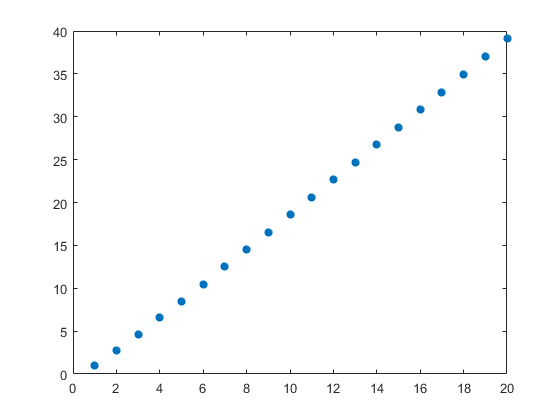
\includegraphics[width = .60\textwidth]{logvander.png}  
  \centering
\end{figure}









\item If everything has gone well, your plot will look like a straight line!  Use a least squares method to find $m$ and $b$ such that
\[
\log(\kappa_n) \approx m n + b
\]
Then plot your line on the same graph as in part (b).\\

\textbf{Console:}
\begin{center}
\lstinputlisting{leastvander.txt}
\end{center}


\begin{figure}[h]
  \caption{Plot of $log(\kappa_n)$ over $n$ (red)  and $\log(\kappa_n) \approx 2.02n - 1.50$ (blue)}
  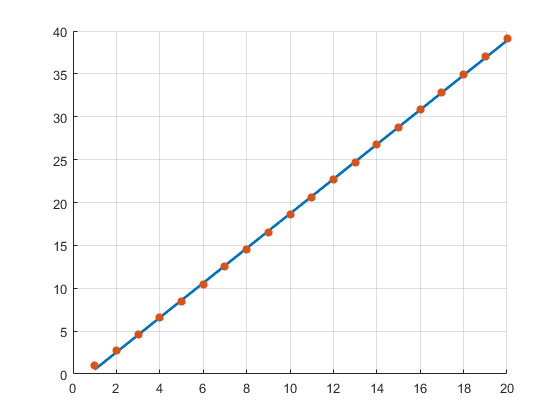
\includegraphics[width = .60\textwidth]{leastvander.png}  
  \centering
\end{figure}

\item Find constants $C$ and $\alpha$ such that
\[
\kappa_n \approx C \alpha^n
\]\\
\solution From Supplemental 2 we know that $C = e^b$ and $\alpha = e^M$ so plugging in our values for $M$ and $b$ that 
we solved for in the previous problem we get that,
\begin{equation*}
  C = e^{1.50} \approx 0.2228,
\end{equation*}  
\begin{equation*}
  \alpha = e^{2.02} \approx  7.5336.
\end{equation*}  


\end{enumerate}
\end{exercise}

\end{document}